% Maintain the consistency.
% Maintain a good writing flow. 

\section{Introduction}\label{sec:introduction}
One of the most significant advantages of employing technologies over analogue processes is that it is less expensive in terms of time. Conventionally, we continue to do all of the official activities, including fees payment as well as attendance, via the use of paper documents. In addition to increasing time consumption, it also makes students more reliant on authority and the particular time limits imposed by the authorities. Furthermore, there is always the possibility of unsuccessful finishing of the task. Considering these circumstances, our objective is to create an application that will transfer these two procedures (payment and attendance system) to a digital platform, which will be able to complete the duties in the shortest amount of time imaginable and with the least amount of paperwork possible. The system will provide students with independence from the tormenting limits of the administration while also allowing the authorities to make their duties more manageable for themselves. For both students and administrators, it goes without saying that the system would be user-friendly in its design.\\

This document is a record of a strategic and creative process that was focused on clearly describing concerns and objectives, as well as providing an overview of the application that represented the narrative from the beginning to the completion of the process. Anyone interested in using or developing the system would be able to do so with the assistance of this documentation.

%The purpose of this course is to develop a database application system by applying the theories, methodologies, tools, and technologies we learnt in CSE 413 that is Database System course.%  

\clearpage


\subsection{Background and Motivation}\label{subsec:bm}

Every year since the university’s founding in 1966, students have increased by a small but steady margin. Even though the globe is being exposed to new technology daily, the method for receiving fees and the attendance system at the University of Chittagong have stayed the same. The dependency on a single branch of a single bank makes the payment process of tuition fees difficult to manage not only for students but also for the administration. Students despise this analogue approach, especially since they are restricted to a one-day time frame to deposit the money during class days or in the weeks leading up to the test. As the number of students continues to rise year after year, university administrators and bank administrators have had enough of this terrible procedure. The same may be said regarding the old method of attendance. 25 to 30 percentile of a class period is devoted to traditionally attesting attendance.


If we take a closer look, we can see that these issues are interconnected. We want to create a system to tackle these difficulties while also processing primary data from both students and instructors. The system does not need paperwork to accomplish the functions and demands the most negligible physical presence from authorities and students. This system will convert both the payment and attendance systems to a one-click operation. Administrators' capability to query the necessary information will be more accessible than ever before. Students and administrators may use this system to run processes from any location, with an immediate time stamp to validate them.

\subsection{Problem Statement}\label{subsec:ps} 

\emph{Develop a database system to handle online fees payment and attendances.}

The system may use student data such as \emph{name}, \emph{student id}, some institutional data such as \emph{course}, \emph{department}, some teacher's data such as \emph{teacher's name}, \emph{the department he belongs to} and \emph{which courses he teaches} and so on. The system needs to hold the records of payments already done and have to be done by a student. Also, implement an online attendance system using the information of courses from a teacher and the students studying the course on the same platform.

\clearpage

\subsection{System Definition}\label{subsec:sd} 

\textit{Generally, an online application uses the internet, and users can have access globally. According to requirements, we are supposed to implement an online application named ``Chittagong University Online Payment and Attendance System (CU-OPAS)." It will manage the student fees and attendances. A digital platform-based system will save time and provide a paperless working facility.}


\subsection{System Development Process}\label{subsec:sdp}

To develop our system, we use the system development life cycle (SDLC) process [https://g.co/kgs/nFcYCv]. Figure~\ref{fig:sdlc} shows the different steps of the SDLC process: Requirement Gathering, Requirement Analysis, Database Modeling, Architectural Design, Implementation, and Testing and Validation. It is a cyclic process and allows to include new requirements given by uses at the validation stage. SDLC provides an effective method and framework to develop a system. It also provides enables project planning, scheduling and estimating. As a result, developers can estimate costs and have proper planning for project tracking and control. This increases the development speed and enables developers to design and build a high-quality system. Considering all of these facilities, we've chosen it.

\begin{figure}[H]
    \centering
    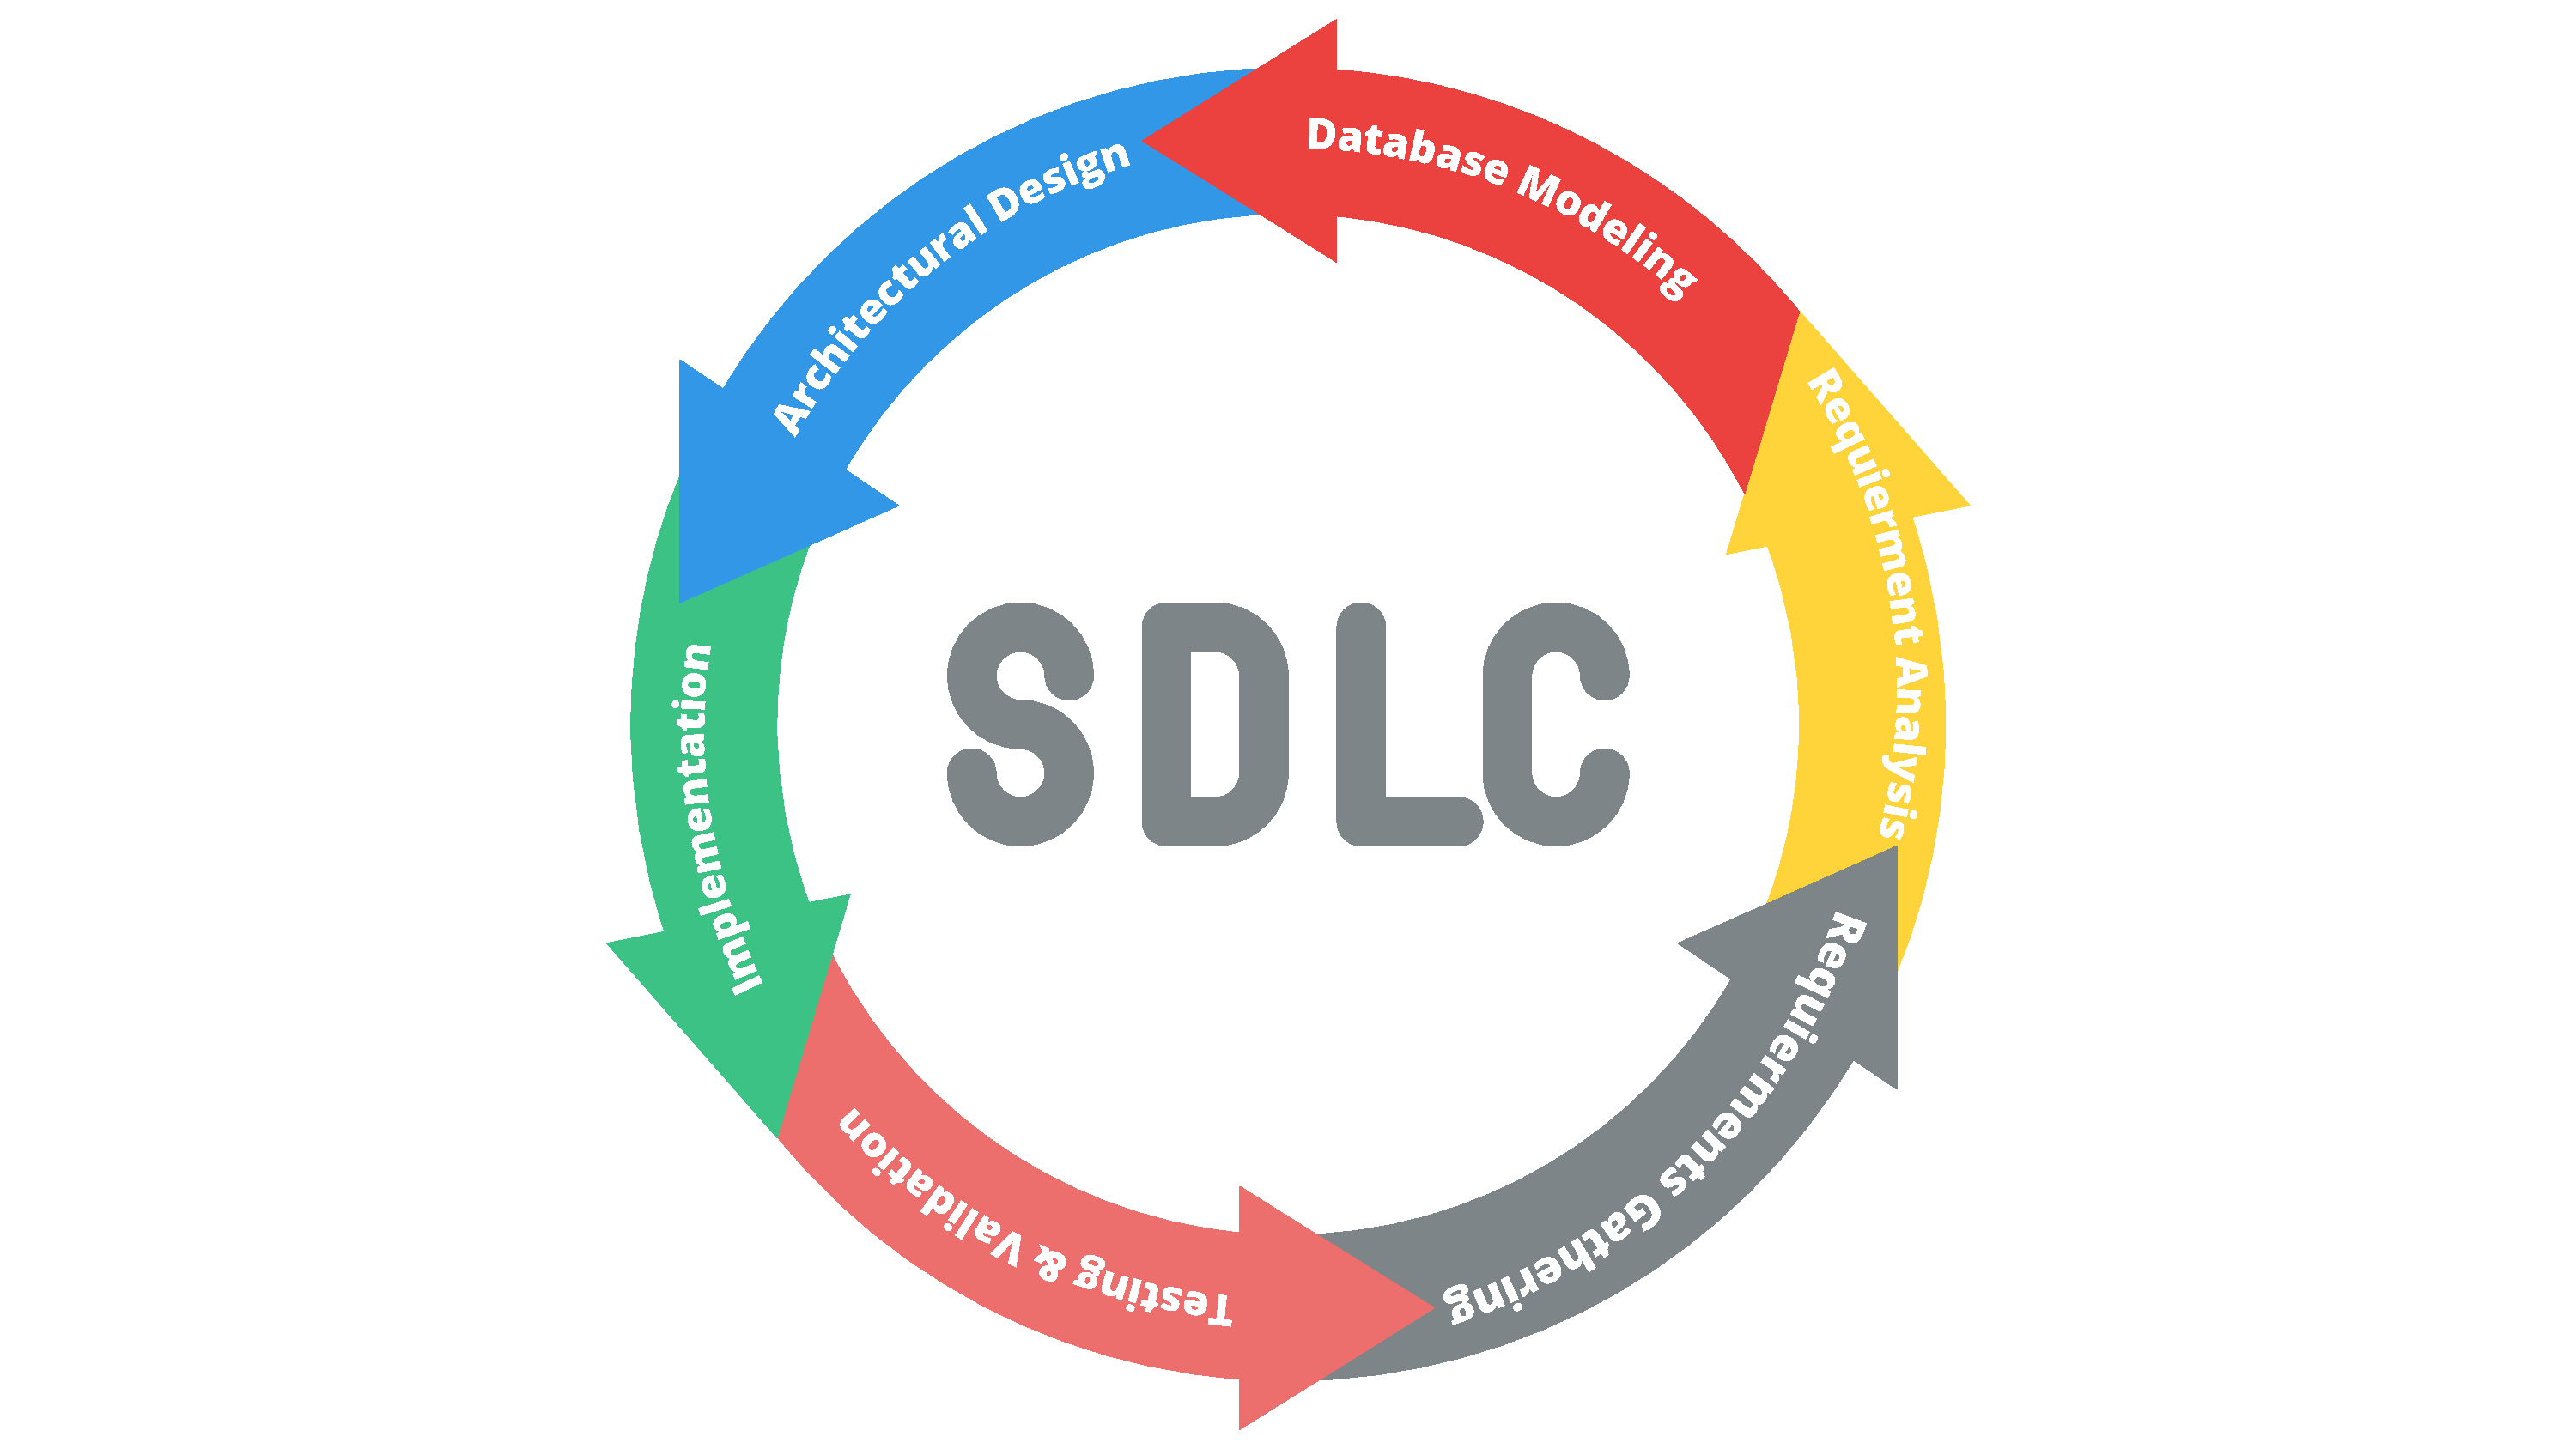
\includegraphics[width=1\textwidth]{images/sdlc}
    \caption{System Development Life Cycle (SDLC)}
    \label{fig:sdlc}
\end{figure}

In the following, we briefly define the each step.
\begin{description}
\item [Requirement Gathering] The requirements collection and analysis step is the most critical element of the whole process. It is at this phase that the client explains his or her expectations for the project, including who will use the product, how the customer will use the product and the specific data that will be included with any unusual client needs that have been recognized. Project managers often use a variety of approaches to gather the requirements for their projects. Interviews, surveys, observations, and workshops are some of the most well-known types of research methods. We employed interview and questionnaire methodologies to gather the requirements because we were determined to do so.
\item[Requirement Analysis] The research of requirements is vital, as is the basic movement that occurs once the requirements are gathered. We disassemble, improve, and study the needs that have been gathered in order to generate predictable and clear requirements. As part of this effort, all requirements are audited, and a graphical view of the whole framework is provided. Afterwards, when the assessment has been completed, it is common for the task's understandability to significantly increase in terms of comprehension. In this case, we may also make use of the client's relationship to describe areas of disarray and determine which needs are of more importance than others.
\item[Database Modeling] When it comes to database modelling, it's also referred to as data modelling since it involves establishing a data model for the data that will be kept in the database. The third phase of the SDLC is known as the design phase. This data model is a conceptual representation of data items, the connections that exist between them, and the rules that govern them. The Data Model is defined as a theoretical model that organizes information representation, information semantics, and consistency limits of the information in a way that is understandable to the user. The information model emphasizes what information is necessary and how it should be organized, rather than what actions will be done on it, as opposed to the tasks themselves.\\

There are basically three types of data models. These are conceptual data models, logical data models, and physical data models,  each with a specific purpose. [www.en.wikipedia.org/wiki/Data\_model].\\

\begin{itemize}
  \item The conceptual data model mainly defines what the system contains. This model is commonly created by business stakeholders and Data Architects. The intention is to put together, scope, and characterize business ideas and rules.
  \item The logical data model defines how the system should be implemented independently of the DBMS. This model is regularly made by Data Architects and Business Analysts. The object is to foster a specialized guide of rules and information structures.
  \item The physical data model depicts how the system gonna be implemented using a particular DBMS. This model is commonly made by DBA and engineers. The intention is the actual implementation of the database.
\end{itemize}
\item[Architectural Design] The architecture of a system describes its major components, their relationships (structures), and how they interact with each other. It encompasses all of the system's components, as well as subsystems that handle all of the system's operations in their entirety. Figure~\ref{fig:archi} shows the architectural design of Chittagong University Online Payment and Attendance System's (CU-OPAS) architectural design.

\begin{figure}[H]
    \centering
    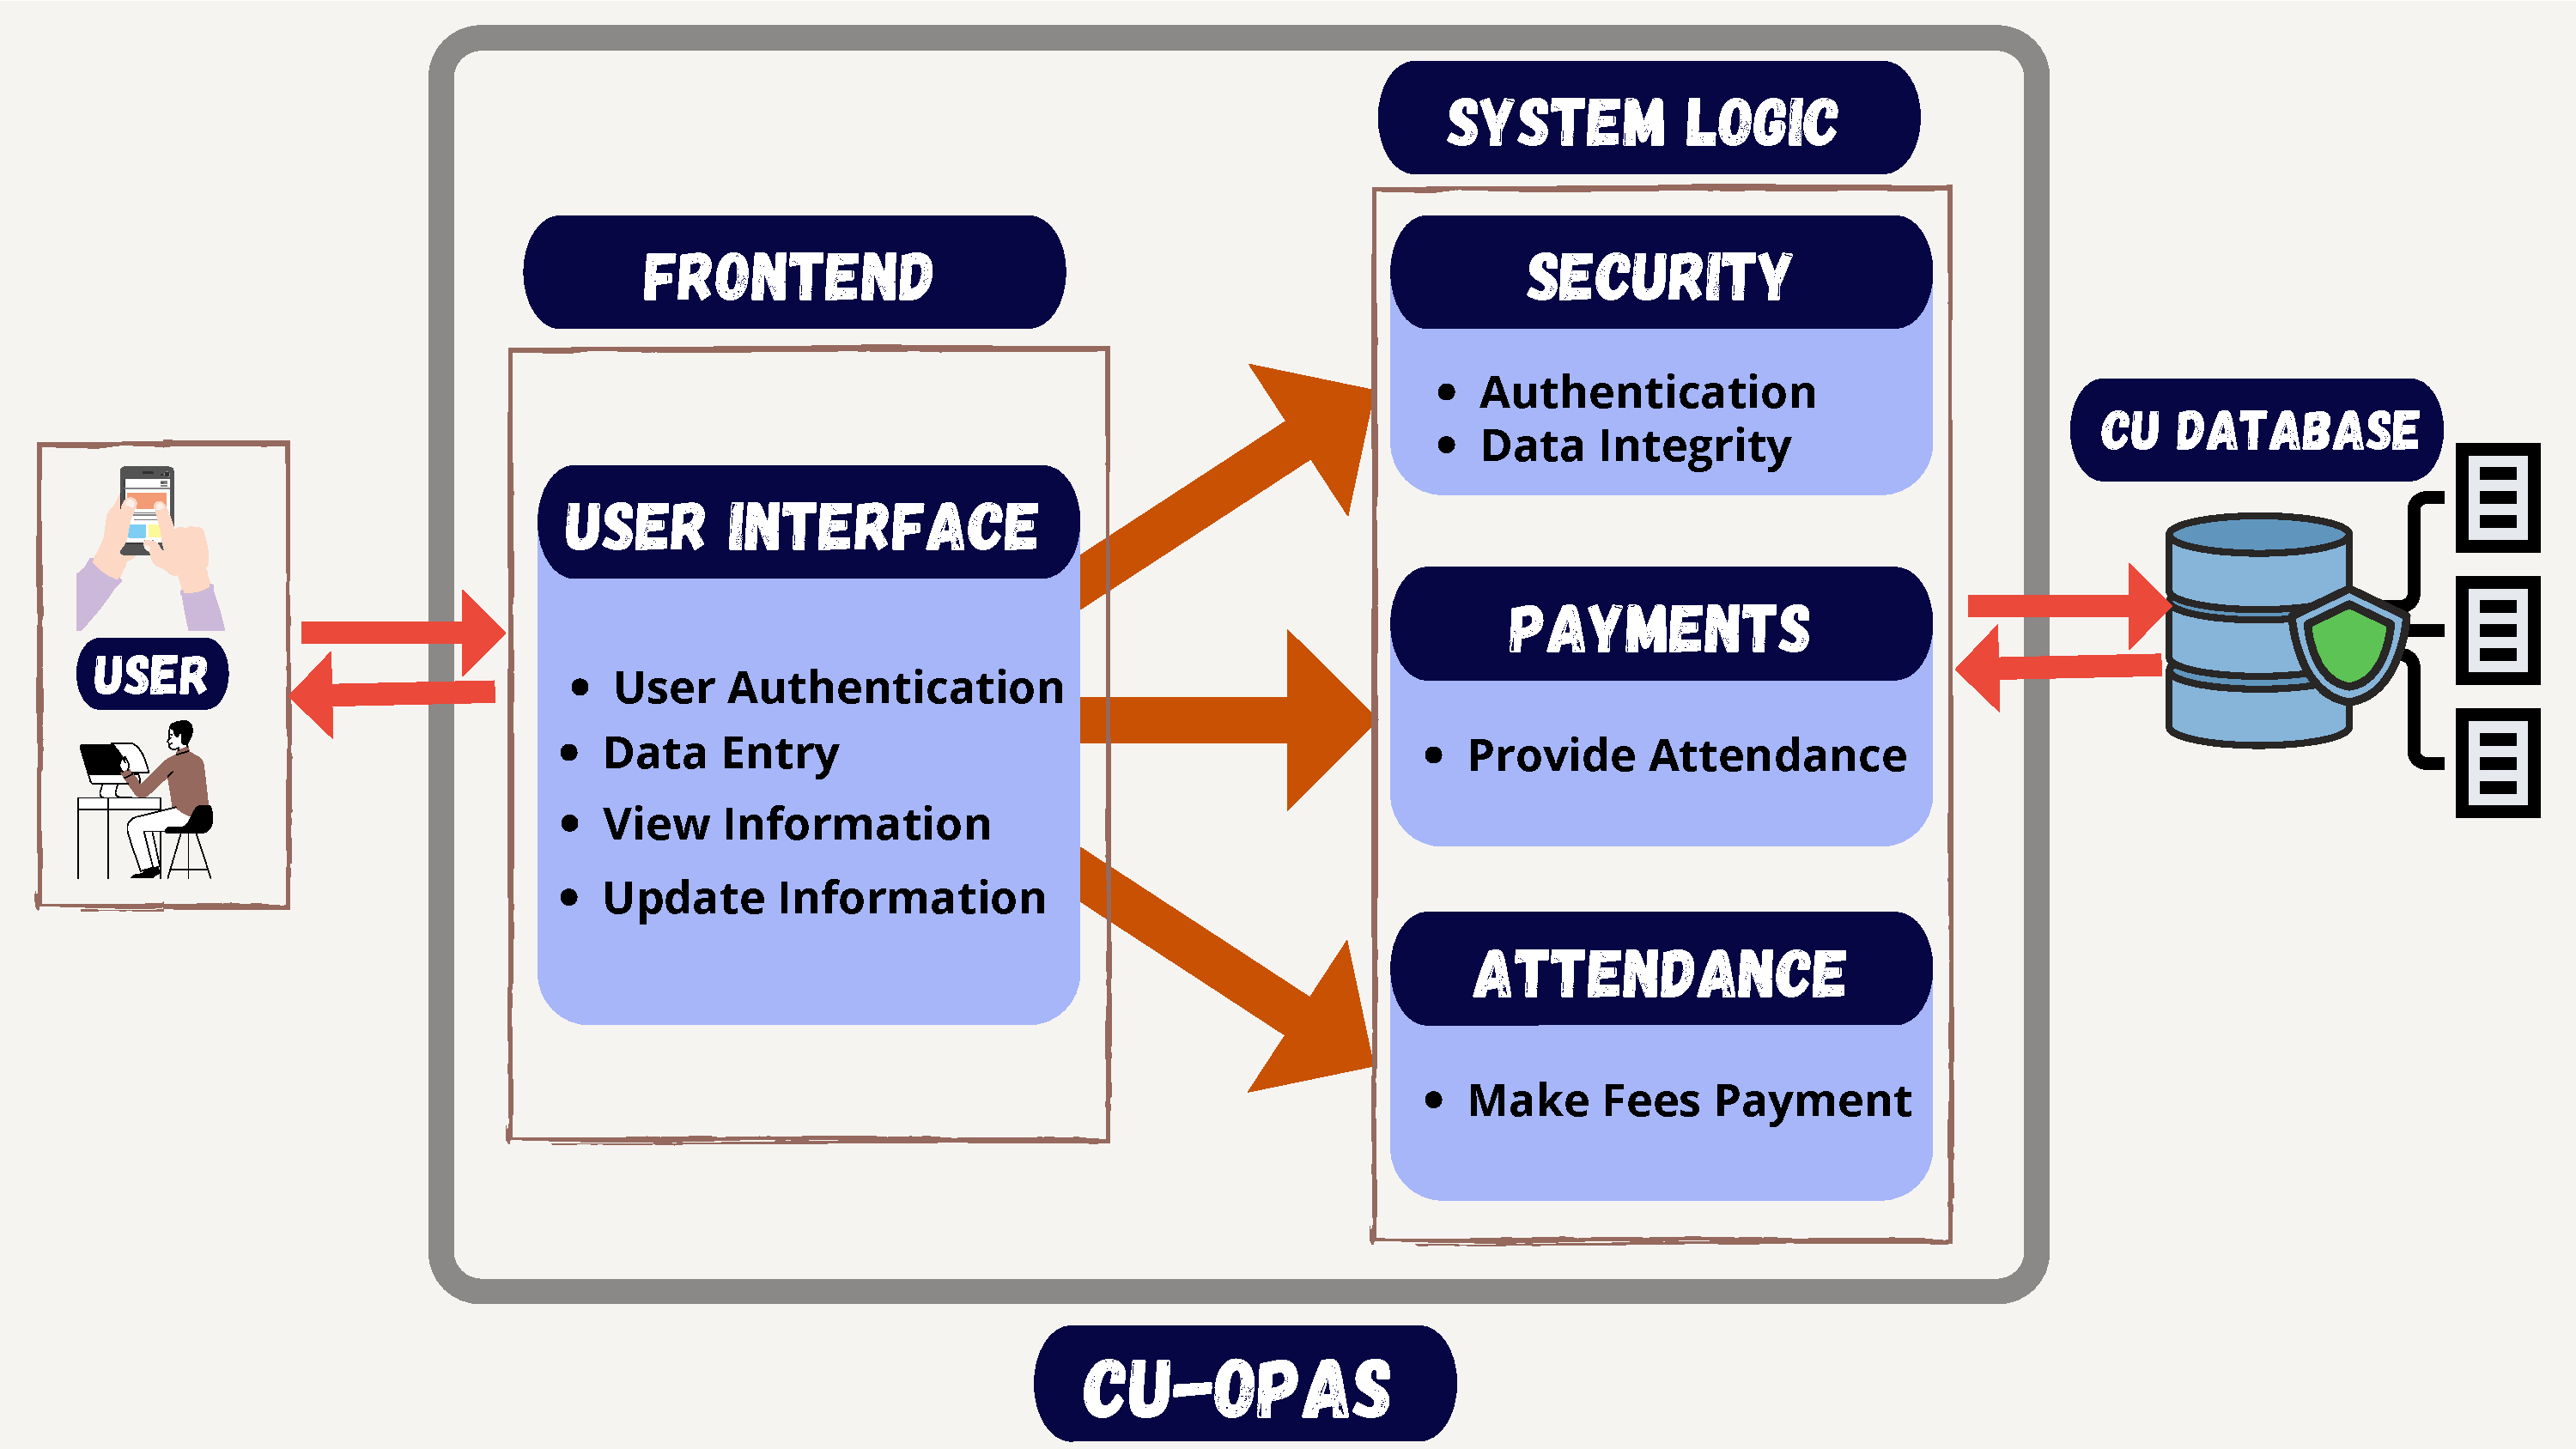
\includegraphics[width=1\textwidth]{images/archi}
    \caption{Architectural design of CU-OPAS}
    \label{fig:archi}
\end{figure}

CU-OPAS(Chittagong University Online Payment and Attendance System) uses request-response patterns to communicate with users. Any legitimate user of this system may request inquiries about payment and attendance activities from the system front-end. Then the system generates a response communicating with the database, as shown in the figure.

\item[Implementation] The implementation process starts when the architectural design and user testing have been completed successfully. It is at this phase that the physical design of the system is completed. It is the third phase of the SDLC. As part of this phase, we employed a range of programming languages, frameworks, tools, and online resources to construct our system from scratch.
\item[Testing and Validation] The final and most crucial phase of the SDLC is validation. This step is critical in ensuring that not just the proper product, but also a high-quality product is produced. Validation can determine whether or not the system meets end-user requirements. We've tested our system in a variety of ways for this aim, including Unit Testing, Integration Testing, System Testing, and Acceptance Testing.
\end{description}

\begin{comment}

To design a database, one should follow the following steps:
\begin{enumerate}
\item Requirement analysis
	\begin{itemize}
		\item[-] interviewing, documentation, etc .
	\end{itemize}

\item Mapping onto a conceptual model (conceptual design)
     \begin{itemize}
     	\item[-] ER model
     \end{itemize}
\item Mapping onto a data model (logical design)
	\begin{itemize}
     	\item[-] Relational model, object model etc. 
     \end{itemize}
\item Normalization
\item System Architecture
\item Realization and Implementation (physical design)    
    
\end{enumerate}
\end{comment}


\subsection{Organization}
Section~\ref{sec:introduction} gives an overview of this project. This section also narrates the project from start to the end briefly. Section~\ref{sec:projectmanagement} describes how the project and the resources are managed. The next Section~\ref{sec:rga} refers to the results of the analysis of the information gathered from the surveys, interviews and discussion with some group of students, teachers and administrative officers. The following Section~\ref{sec:cm}, Section~\ref{sec:lm} and Section~\ref{sec:norm} provide an overview of how we designed the database and enhanced it step by step as most as possible. Section~\ref{sec:sa} and Section~\ref{sec:imp} provide information about the whole system structure and how we implemented it. Section~\ref{sec:val} says how we validated the system with real user data with an statistics on consumed time, cost, user satisfaction between the previous system and this system. Section~\ref{sec:sd} is about the process to install and configure the system so that even a non-technical person can use the system easily. Finally, the conclusion and the pointers to the future work are outlined in Section~\ref{sec:cfw}.

\clearpage